\subsection{Proceso Interno 12: Generar Gráficos}

\subsubsection{Objetivo del Proceso}
El propósito principal de la actividad ``Generar Gráficos'' es utilizar los datos preprocesados y formateados del estado del sistema gravitacional para crear o actualizar una representación visual en la pantalla, empleando las funciones específicas de la biblioteca gráfica seleccionada (por ejemplo, \texttt{Matplotlib}, \texttt{Pygame}, \texttt{Plotly}). Esta actividad asegura que el estado del sistema, como las posiciones de las partículas o los valores de energía, se visualice de manera clara y precisa para el usuario, soportando el análisis y monitoreo de la simulación en el contexto del proyecto.

\subsubsection{Entradas Principales}
\begin{itemize}
    \item \textbf{Datos Formateados:}
    Una estructura de datos generada por el proceso ``Procesar Datos'', que contiene información lista para graficar, como:
    \begin{itemize}
        \item Coordenadas para trayectorias (por ejemplo, \texttt{x\_list}, \texttt{y\_list} para 2D, o \texttt{x\_list}, \texttt{y\_list}, \texttt{z\_list} para 3D).
        \item Valores escalares para gráficos de energía (por ejemplo, \texttt{[t, E\_total]}).
        \item Configuración visual adicional (por ejemplo, colores, tamaños, tipos de gráfico).
    \end{itemize}
    \item \textbf{Contexto Gráfico:}
    Acceso al lienzo, ventana, o superficie de dibujo proporcionada por la biblioteca gráfica, que sirve como el área donde se renderizará la visualización.
\end{itemize}

\subsubsection{Sub-pasos Secuenciales}
Este apartado es proporcionado para profundizar y describir de forma textual cada paso contenido dentro del diagrama del proceso descrito en la figura~\ref{fig:process_diagram12}
\subsubsection*{Recibir Datos Formateados}
\begin{itemize}
    \item La actividad recibe la estructura de datos formateada, que contiene las coordenadas, valores derivados (como energía), y parámetros visuales necesarios para generar el gráfico.
\end{itemize}

\subsubsection*{Preparar Lienzo}
\begin{itemize}
    \item \textbf{Verificar si es Actualización de Frame:}
    \begin{itemize}
        \item Se evalúa si el gráfico es una actualización de un frame anterior (como en una animación) o el primer dibujo en el lienzo.
    \end{itemize}
    \item \textbf{Si es una actualización:}
    \begin{itemize}
        \item Se limpia el área del gráfico anterior para evitar superposiciones. Esto puede implicar:
        \begin{itemize}
            \item Rellenar el fondo con un color sólido (por ejemplo, blanco o negro).
            \item Eliminar objetos gráficos previos (por ejemplo, puntos o líneas) del buffer.
        \end{itemize}
    \end{itemize}
    \item \textbf{Si es la primera vez o no es animación:}
    \begin{itemize}
        \item Se verifica que el lienzo esté inicializado y listo para dibujar, sin necesidad de limpieza.
    \end{itemize}
    \item Esta preparación asegura que el lienzo esté en un estado adecuado para el nuevo dibujo.
\end{itemize}

\subsubsection*{Configurar Parámetros de Visualización}
\begin{itemize}
    \item Se establecen los parámetros gráficos definidos en la configuración, como el estilo de los puntos, colores, tamaños, o propiedades del gráfico (por example, escala de ejes, títulos).
    \item Estos parámetros se pasan a las funciones de dibujo de la biblioteca gráfica.
\end{itemize}

\subsubsection*{Llamar Funciones de Dibujo de la API Gráfica}
\begin{itemize}
    \item \textbf{Dibujar Elementos Principales (Partículas):}
    \begin{itemize}
        \item Se utilizan los datos formateados para dibujar los elementos primarios, como las partículas. Por ejemplo:
        \begin{itemize}
            \item Para una trayectoria 2D, se llama a funciones como \texttt{draw\_circle~()} (\texttt{Pygame}) o \texttt{scatter~()} (\texttt{Matplotlib}) para cada partícula, usando coordenadas \texttt{x\_list} y \texttt{y\_list}.
            \item El tamaño o color de los puntos puede reflejar la masa de las partículas, según la configuración.
        \end{itemize}
    \end{itemize}
    \item \textbf{Dibujar Líneas de Trayectoria o Energía:}
    \begin{itemize}
        \item Se dibujan líneas o curvas que conectan puntos para representar trayectorias o series temporales. Por ejemplo:
        \begin{itemize}
            \item Para trayectorias, se usa \texttt{plot~()} o \texttt{draw\_line~()} para conectar posiciones consecutivas.
            \item Para gráficos de energía, se usa \texttt{plot\_line~()} para añadir un punto (\texttt{[t, E\_total]}) a la serie temporal.
        \end{itemize}
    \end{itemize}
    \item \textbf{Dibujar Elementos Auxiliares (Vectores):}
    \begin{itemize}
        \item Si los datos incluyen velocidades y la configuración lo requiere, se dibujan vectores de velocidad usando funciones como \texttt{draw\_line~()} o \texttt{arrow~()} para cada partícula.
    \end{itemize}
    \item \textbf{Agregar Elementos Contextuales:}
    \begin{itemize}
        \item Se añaden elementos gráficos como ejes, etiquetas, títulos, y leyendas, utilizando funciones como \texttt{set\_xlabel~()}, \texttt{set\_title~()}, o \texttt{add\_legend~()} en la API gráfica.
    \end{itemize}
    \item Cada llamada a la API utiliza los datos formateados como argumentos, asegurando que la representación visual sea precisa.
\end{itemize}

\subsubsection*{Actualizar/Refrescar Pantalla}
\begin{itemize}
    \item Una vez que todos los elementos gráficos han sido dibujados en el buffer gráfico, se llama a la función de la biblioteca gráfica que hace visible el buffer en la pantalla. Por ejemplo:
    \begin{itemize}
        \item \texttt{pygame.display.flip~()} en \texttt{Pygame}.
        \item \texttt{plt.draw~()} o \texttt{fig.show~()} en \texttt{Matplotlib}.
        \item \texttt{plotly.render~()} en \texttt{Plotly}.
    \end{itemize}
    \item Esto asegura que el usuario vea la representación gráfica actualizada.
\end{itemize}

\subsubsection*{Liberar Recursos Temporales (Si Aplica)}
\begin{itemize}
    \item Se liberan recursos temporales utilizados durante el dibujo, como buffers intermedios o estructuras de datos auxiliares, para optimizar el uso de memoria.
    \item En la mayoría de los casos, las bibliotecas gráficas manejan esta limpieza automáticamente.
\end{itemize}

\subsubsection{Lógica Interna y Decisiones}
\begin{itemize}
    \item \textbf{Actualización vs\. Primer Dibujo:}
    La decisión de limpiar el lienzo depende de si el gráfico es una actualización en una animación o un dibujo inicial. Esta bifurcación asegura que las animaciones no acumulen artefactos visuales de frames anteriores.
    \item \textbf{Tipo de Elementos Gráficos:}
    La selección de funciones de dibujo (por ejemplo, \texttt{scatter} para partículas, \texttt{plot} para líneas) depende implícitamente del tipo de gráfico especificado en los datos formateados (trayectoria, energía, etc.).
    \item \textbf{Elementos Auxiliares:}
    La inclusión de vectores de velocidad, etiquetas, o leyendas es condicional, basada en la configuración visual y la disponibilidad de datos (por ejemplo, velocidades).
    \item \textbf{Manejo de Errores Implícito:}
    Errores como formatos de datos incompatibles con la API gráfica o fallos en el lienzo son manejados por la biblioteca gráfica, que puede lanzar excepciones. Esta actividad asume que los datos formateados son válidos, gracias al procesamiento previo.
\end{itemize}

\subsubsection{Manejo de Datos Específico}
\begin{itemize}
    \item \textbf{Datos de Entrada:}
    \begin{itemize}
        \item Estructura de datos formateada (por ejemplo, \texttt{x\_list}, \texttt{y\_list}, \texttt{[t, E\_total]}) con coordenadas, valores escalares, y parámetros visuales.
        \item Contexto gráfico (lienzo o ventana de la biblioteca gráfica).
    \end{itemize}
    \item \textbf{Datos Intermedios:}
    \begin{itemize}
        \item Ningún dato numérico nuevo se genera; los datos formateados se consumen directamente como parámetros para las funciones de dibujo.
    \end{itemize}
    \item \textbf{Datos de Salida:}
    \begin{itemize}
        \item No se generan datos numéricos como salida; el resultado es la modificación del buffer gráfico, que produce una representación visual en la pantalla.
    \end{itemize}
\end{itemize}

\subsubsection{Salidas Principales}
\begin{itemize}
    \item \textbf{Representación Gráfica Actualizada:}
    La visualización del estado del sistema (por ejemplo, posiciones de partículas, trayectorias, o gráficos de energía) renderizada y visible en la interfaz gráfica, proporcionando al usuario una representación clara del comportamiento dinámico.
\end{itemize}

\subsubsection{Interacciones Internas}
\begin{itemize}
    \item \textbf{Con el Proceso Anterior:}
    Recibe los datos formateados del proceso ``Procesar Datos''.
    \item \textbf{Con la Biblioteca Gráfica:}
    Interactúa extensamente con la API de la biblioteca gráfica (por ejemplo, \texttt{Matplotlib}, \texttt{Pygame}, \texttt{Plotly}) para dibujar elementos y actualizar la pantalla.
    \item \textbf{Con el Lienzo Gráfico:}
    Modifica el estado del lienzo o ventana gráfica, ya sea limpiándolo, dibujando nuevos elementos, o refrescando el buffer para mostrar la visualización.
    \item \textbf{Con el Pipeline de Visualización:}
    Completa el flujo de visualización, transformando los datos formateados en una salida gráfica que el usuario puede observar.
\end{itemize}
\newpage
\subsubsection{Diagrama del Proceso}
\begin{figure}[H]
    \centering
    \adjustbox{max width=\textwidth, max height=0.9\textheight}{%
    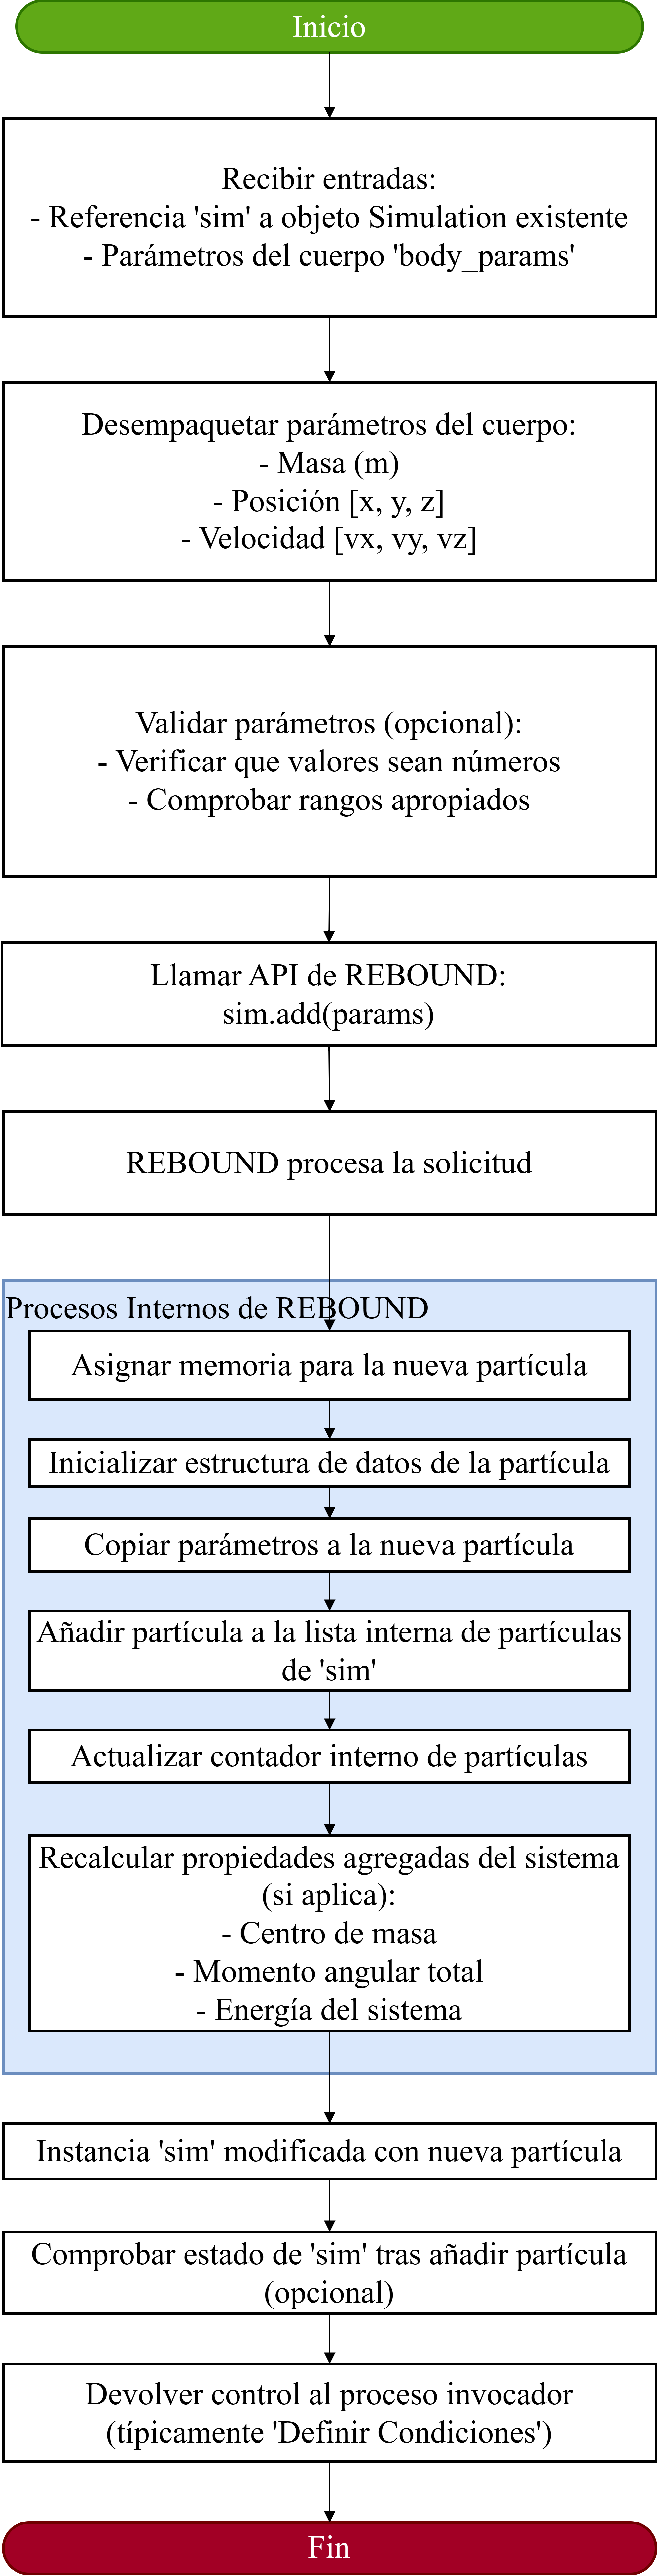
\includegraphics{img/Analisis/DiagramaProcesos/DiagramaProceso05AgregarCuerpos.png}
    }
    \caption{Diagrama de Proceso Interno 05: Agregar Cuerpos}%
    \label{fig:process_diagram05}
\end{figure}
\newpage